\chapter{Versicherung}
\label{chap:Versicherung}
Im Bereich Versicherung gibt es mehrere Bestrebungen, mithilfe von Smart Contracts die automatische Abwicklung von Versicherungsfällen zu regeln. Die 2018 gegründete B3i Initiative, hinter der namhafte Versicherungsunternehmen wie Zurich, AXA, Generali und die Allianz stehen, hat sich zur Aufgabe gemacht, Standards für die Branche zu entwickeln und das nötige Netzwerk und die Anwendungen aufzubauen \cite[vgl.][]{B3iWhoWeAre2019}. Da die Applikation erst im Juli 2019 startet \cite[vgl.][]{B3iHackathon2019}, eignet es sich nicht, um tiefer darauf einzugehen.

Eine bereits lauffähige Anwendung auf der Ethereum Blockchain existiert mit fizzy, einer Applikation von AXA. Fizzy sichert Personen gegen Flugzeugverspätungen bei mehr als zwei Stunden oder kompletter Annulierung des Fluges ab. Mit Anlegen einer Versicherung, was bis spätestens fünf Tage vor Abflug möglich ist, wird die Fluginformation an einen Smart Contract weitergegeben, welcher die Daten in der Blockchain speichert. Durch eine Koppelung an Flugdaten wird der Betrag im Versicherungsfall innerhalb einer Standard-Bankenlaufzeit ausbezahlt. Die Gebühren für die Absicherung werden dabei von einem Algorithmus anhand des Flug-Ausfallsrisikos berechnet. Durch den Einsatz von Blockchain-Technologie wird auf beiden Seiten Transparenz und Unveränderlichkeit der Bedingungen garantiert. \cite[vgl.][]{Fizzy2019}

Da fizzy mit \cite{Clement2019} einen Artikel bereitgestellt hat, um einen besseren Einblick in den zugrundeliegenden Smart Contract zu bekommen, wird im Folgenden ein Beispiel besprochen.\\
Seit 22. Mai 2019 gibt es eine neue Variante des Smart Contracts \cite{EtherscanNewContract2019}, welcher mit 742 Zeilen Solidity Code deutlich mehr Funktionalität liefert, als der ursprüngliche Smart Contract mit gerade einmal etwas mehr als 200 Codezeilen \cite{EtherscanOldContract2019}. Zur Betrachtung wird nun in Teilen der neue Contract herangezogen.

\begin{figure}[h!]
  \centering
  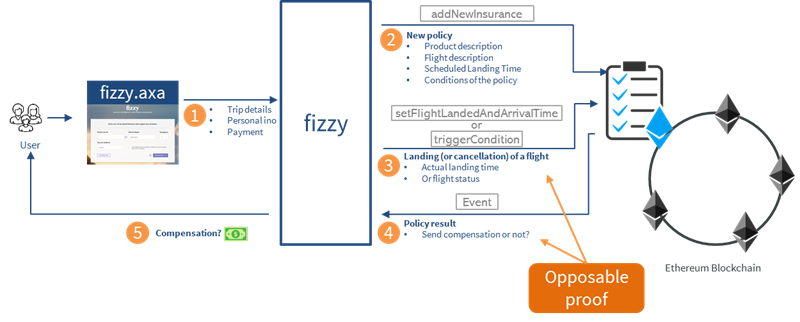
\includegraphics[width=\textwidth]{Bilder/fizzyAblauf.png}
  \caption[Ablauf fizzy Smart Contract]{Ablauf fizzy Smart Contract \cite{Clement2019}}
  \label{fig:fizzyAblauf}
\end{figure}

